%% ****** Start of file aiptemplate.tex ****** %
%%
%%   This file is part of the files in the distribution of AIP substyles for REVTeX4.
%%   Version 4.1 of 9 October 2009.
%%
%
% This is a template for producing documents for use with 
% the REVTEX 4.1 document class and the AIP substyles.
% 
% Copy this file to another name and then work on that file.
% That way, you always have this original template file to use.

\documentclass[aip,amsmath,amssymb,reprint,floatfix]{revtex4-1}
%\documentclass[aip,reprint]{revtex4-1}

\usepackage{graphicx}% Include figure files
\usepackage{dcolumn}% Align table columns on decimal point
\usepackage{bm}% bold math
%\usepackage[mathlines]{lineno}% Enable numbering of text and display math
%\linenumbers\relax % Commence numbering lines

% hyphenation
\usepackage{hyphenat}
%\usepackage{lipsum}

% tables
%\usepackage{dcolumn}
\usepackage{multirow}
%\usepackage{hhline}
\usepackage{booktabs}
%\usepackage{longtable}

% mathematics
\usepackage{amsmath}
\usepackage{amsfonts}
\usepackage{amssymb}
\usepackage{amsbsy}
%\usepackage{bm}
\usepackage{mathrsfs}
\usepackage{upgreek}
%\allowdisplaybreaks

% symbols
%\usepackage{gensymb}
%\usepackage{textcomp}

%---------------------------------------------------
% happy integral
\newcommand{\rint}[1]{\mbox{\Large $ \int\limits_{\mbox{\tiny  $#1$}}$}}
% SHORTCUTS
%\newcolumntype{,}{D{.}{,}{2}}
\newcommand{\citee}[1]{\ensuremath{\scriptsize^{\citenum{#1}}}}
\newcommand{\HRule}{\rule{\linewidth}{0.2mm}}
% Quantum notation
\newcommand{\bra}[1]{\ensuremath{\bigl\langle {#1} \bigl\lvert}}
\newcommand{\ket}[1]{\ensuremath{\bigr\rvert {#1} \bigr\rangle}}
\newcommand{\braket}[2]{\ensuremath{\bigl\langle {#1} \bigl\lvert {#2} \bigr\rangle}}
\newcommand{\tbraket}[3]{\ensuremath{\bigl\langle {#1} \bigl\lvert {#2} \bigl\lvert {#3} \bigr\rangle}}
% Math
\newcommand{\pd}{\ensuremath{\partial}}
\newcommand{\DR}{\ensuremath{{\rm d} {\bf r}}}
%\newcommand{\BM}[1]{\ensuremath{\mbox{\boldmath${#1}$}}}
\newcommand{\BM}[1]{\bm{#1}}
% Chemistry (formulas)
\newcommand{\ch}[2]{\ensuremath{\mathrm{#1}_{#2}}}
% Math 
\newcommand{\VEC}[1]{\ensuremath{\mathrm{\mathbf{#1}}}}
% vector nabla
\newcommand{\Nabla}{\ensuremath{ \BM{\nabla}}}
% derivative
\newcommand{\FDer}[3]{\ensuremath{
\bigg(
\frac{\partial #1}{\partial #2}
\bigg)_{#3}}}
% diagonal second derivative
\newcommand{\SDer}[3]{\ensuremath{
\biggl(
\frac{\partial^2 #1}{\partial #2^2}
\biggr)_{#3}}}
% off-diagonal second derivative
\newcommand{\SSDer}[4]{\ensuremath{
\biggl(
\frac{\partial^2 #1}{\partial #2 \partial #3}
\biggr)_{#4}}}
% derivatives without bound
% derivative
\newcommand{\fderiv}[2]{\ensuremath{
\frac{\partial #1}{\partial #2}}}
% diagonal second derivative
\newcommand{\sderiv}[2]{\ensuremath{
\frac{\partial^2 #1}{\partial #2^2}
}}
% off-diagonal second derivative
\newcommand{\sderivd}[3]{\ensuremath{
\frac{\partial^2 #1}{\partial #2 \partial #3}
}}
% derivatives for tables
\newcommand{\fderivm}[2]{\ensuremath{
{\partial #1}/{\partial #2}}}
% diagonal second derivative
\newcommand{\sderivm}[2]{\ensuremath{
{\partial^2 #1}/{\partial #2^2}
}}
% off-diagonal second derivative
\newcommand{\sderivdm}[3]{\ensuremath{
{\partial^2 #1}/{\partial #2 \partial #3}
}}
% ERIs and OEIs
\newcommand{\OEIc}[3]{\ensuremath{\left(#1 \lvert #2 \rvert #3 \right)}}
\newcommand{\ERIc}[4]{\ensuremath{\left(#1 #2 \vert #3 #4 \right)}}

% Partial density and potential
\newcommand{\PartPot}[4]{\ensuremath{\frac{#1 #2}{\lvert #3-#4 \rvert }}}

% trace operator
\DeclareMathOperator{\Tr}{Tr}

%\draft % marks overfull lines with a black rule on the right

\begin{document}

\preprint{AIP/123-DMS}

\title{One-Particle Density Matrix Polarization Susceptibility Tensors}

\author{Bartosz B{\l}asiak}
\email[]{blasiak.bartosz@gmail.com}
\homepage[]{https://www.polonez.pwr.edu.pl}
%\thanks{Bulak}
\affiliation{Department of Physical and Quantum Chemistry, Faculty of Chemistry, Wroc{\l}aw University of Technology, Wybrze{\.z}e Wyspia{\'n}kiego 27, Wroc{\l}aw 50-370, Poland}

\date{\today}

\begin{abstract}

%Considering the solvent effect on the correlated electronic wavefunctions, especially
%those that describe the electronically excited state, is a great challenge of Quantum Chemistry. 

In this work, the electric field\hyp{}induced change in the one\hyp{}electron density
has been expressed as a series of the one\hyp{}particle density matrix susceptibility tensors
interacting with electric fields. The analytical approximate expressions were derived
at the Hartree\hyp{}Fock theory, which served as a basis for construction of generalized
model that can be used for an arbitrary form of wavefunction as long as the one\hyp{}particle
density matrices are available. It is shown that it is possible to accurately predict the changes
in the one\hyp{}electron density of water molecule in spatially non\hyp{}uniform electric field distribution
generetated by point charges. The electric field\hyp{}induced interaction energies,
dipole moments and quadrupole moments
are quantitatively described by the present theory in weak and moderate electric fields (0.003 -- 0.02 a.u.).
%It is believed that the possibility of extension of the proposed model with high\hyp{}order susceptibilities
%opens new routes in quantum chemistry of fast and efficient calculations of strongly perturbed systems.
It is believed that the proposed model, after extensive development on its optimization, could open
new routes in quantum chemistry of fast and efficient calculations of strongly perturbed systems.
\end{abstract}

\pacs{}% insert suggested PACS numbers in braces on next line

\maketitle %\maketitle must follow title, authors, abstract and \pacs

\section{\label{s:1}Introduction}

Molecular\hyp{}level exploration of condensed phase phenomena becomes increasingly unavoidable
as technology and medicine continue to develop. Unfortunately, the computational cost of accurate
electronic structure calculations grows extremely fast with the number of particles, greatly limiting
the use of the state\hyp{}of\hyp{}the\hyp{}art first\hyp{}principles theories 
when large and complex chemical systems such as
solutions and biomolecules come into play.\cite{Tomasi.Mennucci.Cammi.ChemRev.2005}
%Although the advent in the computer technology 
%brought some hopes, it is still insufficient to follow up the expensive needs
%of computational chemistry.
Due to this reason, it has been of particular importance nowadays 
to develop bridging theoretical techniques that link
extremely accurate but localized pieces of information 
with certain knowledge of an atomistic organisation and intermolecular interaction
on a relatively large spatial scales, typically ranging beyond few nanometers. 

The discovery of hybrid methods such as quantum mechanical\hyp{}molecular mechanical (QM/MM)
technique was a revolution in computational chemistry and allowed insightful theoretical studies
of quantum mechanical effects in biological systems because the high\hyp{}level
and costly quantum mechanical calculations
could be combined with low\hyp{}level and cheap classical dynamics.\cite{Warshel.Levitt.JMolBiol.1976,Senn.Thiel.Angew.2009}
%That was possible due to the fruitful incorporation of accurate \emph{ab initio} methods and a 
%semi\hyp{}classical notion of molecular motion combined with extensive experimental and semi\hyp{}empirical
%refinings.
Understanding physics that rules intermolecular interactions\cite{Jeziorski.Moszynski.Szalewicz.ChemRev.1994} 
helped to develop
a wide family of force fields, and served a basis for embedding Hamiltonian
within an effective environment and fragmentation methods.\cite{Gordon.Fedorov.Pruitt.Slipchenko.ChemRev.2012}
%The size of quantum level can be extended without compromising accuracy and maintaining good performance
%by using vast family of fragmentation methods, such as effective fragment potentials (EFP).
%The most difficult to tackle part of Hamiltonian can also be embedded within a widely understood effective environment
%leading to various embedding methodologies, realising similar goals.

However, even with the modern advances in computational chemistry, 
%accurate description of environmental effects
accurate description of phenomena due to complex heterogeneous molecular environments 
remains a challenge in the following areas: (i) describing the electronically excited states 
(electronic solvatochromism),\cite{Barbati.JACS.2014,
Szabla.Sponer.Jiri.Gora.JPCL.2015,
Bednarska.Zalesny.Tian.Murugan.Agren.Bartkowiak.Molecules.2017,
Jedrzejewska.Grabarz.Bartkowiak.Osmialowski.SpectChimActA.2018} 
(ii) understanding the vibrational properties of molecules in ground and electronically excited states
(vibrational or vibronic solvatochromisms).\cite{Blasiak.Londergan.Webb.Cho.ACR.2017} 
Interface between QM and MM levels is usually realized by electrostatic embedding
and only rarely includes the Pauli exclusion principle and dispersion.\cite{List.Olsen.Kongsted.PCCP.2016}
Unfortunately, it is quite difficult to efficiently treat the environment\hyp{}induced potential operator
because of complicated nature of intermolecular interactions, that theoretically
cannot be solely envisioned as a sum of electrostatic, dispersion and Pauli effects.
Perhaps the most frequently used efficient and accurate \emph{ab initio} fragmentation methods,
the effective fragment potential (EFP) methods, are limited to the ground\hyp{}state
chemistry at the Hartree\hyp{}Fock (HF)\cite{Gordon.Smith.Xu.Slipchenko.AnnuRevPhysChem.2013} 
or density functional theory (DFT) levels\cite{Nguyen.Pachter.Day.JCP.2014},
and, while they can approximately describe the environment composed of molecules in their ground states,
they cannot be used for highly correlated wavefunctions such as electronically excited states.
%Therefore, Hamiltonian embedding is often realised by Coulombic embedding with polarization
%of QM level, and only rarely the Pauli exclusion principle is taken into account. Although
%such approach is very accurate in certain cases, it is not guaranteed that it is sufficient
%for all cases.

Most of efforts to theoretically treat extended molecular aggregates are rooted in 
energy\hyp{} (or force field\hyp{})based philosophy. However,
in the past decade there has been considerable interest in density\hyp{}based approaches
of a wide scope and aims.\cite{Piquemal.Cisneros.Reinhardt.Gresh.Darden.JCP.2006,
Mandado.Hermida-Ramon.JCTC.2011,
Sun.Chan.ACR.2016,
Hedegard.Reiher.JCTC.2016} 
In particular, the importance of
one\hyp{}electron densities in chemistry is well known and acknowledged in the community,
though still not solved exactly.\cite{Holas.March.PhysRevA.1991}
%that seem to have an important advantage over the standard energetic approach.
With connection to the above, it would be incredibly insightful 
to establish a first\hyp{}principles connection bewteen the one\hyp{}particle
density and the perturbation in the environment through introducing the
\emph{density matrix susceptibility} (DMS) tensors. % because knowing the density distribution
%is equivalent to knowing the state of the molecule.
The main postulate of the present Work is that the associated change 
in the one\hyp{}particle density matrix, $\delta {\bf D}$, can be
deconvoluted into a product form of the generalized perturbation susceptibility ${\bf B}_i$
and the environment\hyp{}induced perturbation on a molecule, $\delta {\bf P}_i$,
evaluated at certain site $i$.
%and induced dipole moments $\delta {\BM\upmu}_i$ due to electric fields ${\bf E}_i$ 
%at the centroids of the occupied molecular orbitals,
%
\begin{equation*} \label{e:initial-model}
 \delta {\bf D} \approx \sum_i^{\text{Sites}} \text{[DMS of the $i$th site]} 
  \cdot  \delta {\bf P}_i
  %\rightarrow \sum_i^{\rm occ} {\bf B}^{(i)}_{\mu\nu} \cdot {\bf E}_i \;.
\end{equation*}
%
While $\delta {\bf P}_i$ contain critical information 
about the actual distortion of the electronic cloud,
perturbation susceptibility is assumed to be a property of unperturbed 
molecule and is to be precomputed only once. 
Thus, such DMS could be adapted into an efficient effective 
one\hyp{}electron fragment potential, in principle applicable to an arbitrary
level of theory, as long as the one\hyp{}particle densities are available.
It also means that such a technique would dramatically reduce costs of quantum chemistry calculations
becuase the task of performing full computation on a molecular aggregate
would reduce to much simpler matrix operations.
%
%a simple first\hyp{}principles model for prediction 
%of the perturbation\hyp{}induced one\hyp{}electron density
%change of structurally unrelaxed molecule is proposed here. 

The simplest, yet perhaps the most relevant for chemistry, type of perturbation 
is the electrostatic perturbation.
It is worth mentioning that, at that moment, there is no simple \emph{ab initio}
method of computation of electron deformation densities without considering the entire molecular 
aggregate by using full quantum chemistry calculations.\cite{Horn.Yuezhi.Head-Gordon.JCP.2016,Horn.Head-Gordon.JCP.2015}
In this Work, we explore the susceptibility of the molecule's electronic density distribution
to polarize due to external electrostatic perturbation from first principles. 
The deformation density is expressed in terms
of the one\hyp{}particle density matrix polarization susceptibility tensors 
that are properties of isolated molecules and can be
extracted from quantum chemistry calculations. The focus on the density (matrix) instead of the energy
(scalar) is beneficial since it provides the directional tensor description
of the polarization that could be combined with other effects such as Pauli repulsion 
or dispersion,\cite{Mandado.Hermida-Ramon.JCTC.2011}
in contrast to the standard interaction energy approaches. We show that accurate polarization 
of the one\hyp{}particle density
matrix is achievable and can be realized as long as the one\hyp{}particle density matrices
are available. It is believed that the proposed method
could be a basis for a construction of an 
alternative approach in fragment\hyp{}based
modelling of extended molecular aggregates that is not limitted to the ground state chemistry.

We introduce the necessary theory and derive the \emph{ab initio} density matrix susceptibility model
at the HF approximation\cite{Roothaan.RevModPhys.1951} 
in Section~\ref{s:2}. Subsequently, this model serves as a basis for generalization to the 
arbitrary one\hyp{}electron density with electronic correlation which is derived in Section~\ref{s:2}. 
The implementation details in a computer code as well as the validation procedures are detailed
in Section~\ref{s:3}. We then discuss the performance of the models in Section~\ref{s:4} 
%based on a few small molecules
%in varying electric field distributions. 
Finally, in Section~\ref{s:5} we conclude the presentation with a few 
remarks for future development.

%
%Understanding intricate mechanisms that govern
%the biomachinery of life requires thorough 

\section{\label{s:2}Theory}

The electronic energy of a closed\hyp{}shell molecule is given by the time\hyp{}independent Schr{\"o}dinger equation,
%
\begin{equation}
 E^{(0)} = \tbraket{\Psi^{(0)}}{\mathscr{H}^{(0)}}{\Psi^{(0)}} \;,
\end{equation}
%
where $E$ stands for the total electronic energy, $\Psi$ the electronic wavefunction and $\mathscr{H}$
the Hamiltonian operator. In the above, the superscript $(0)$
denotes the reference or unperturbed state that is assumed to be known.
Under the influence of an external electrostatic perturbation, the total electronic energy
becomes
%
\begin{equation}
 E[{\bf F}({\bf r})] = \tbraket{\Psi}{\mathscr{H}^{(0)} + \mathscr{V}({\bf F}({\bf r}))}{\Psi}
\end{equation}
%
in which ${\bf F}({\bf r})$ is a non\hyp{}uniform electric field distribution.
The electric field\hyp{}induced energy change is an unknown functional 
of the associated change in the one\hyp{}electron density,
%
\begin{equation}\label{e:rho}
 \rho({\bf r}) = 2\sum_{\alpha\beta} D_{\alpha\beta} \phi_\alpha({\bf r}) \phi^*_\beta({\bf r}) \;.
\end{equation}
%
In Eq.~\eqref{e:rho} $\phi_\alpha({\bf r})$ is a basis funtion, which can be for instance 
an atomic orbital (AO) or a molecular orbital (MO), and $D_{\alpha\beta}$ is the corresponding
one\hyp{}particle density matrix.
If perturbation\hyp{}independent basis is chosen, the electric field\hyp{}induced change in the one\hyp{}particle density
is given by
%
\begin{equation}\label{e:rho-1}
 \delta \rho({\bf r}) = 2\sum_{\alpha\beta} \delta D_{\alpha\beta} \phi_\alpha({\bf r}) \phi^*_\beta({\bf r}) \;.
\end{equation}
%
Ideally, the electric field\hyp{}induced change in the ground state's one\hyp{}particle density 
follows its energy minimum of the perturbed state. In addition, all the perturbed 
excited state one\hyp{}electron densities must be excited state solutions of the Schr{\"o}dinger equation
with the exact energy\hyp{}minimized ground state. 

Development of a first\hyp{}principles theory
that is capable of accurately capturing the electric field\hyp{}dependence of the one\hyp{}particle density
is extremely difficult. This is not only because of the very complicated (and generally unknown) solution
to the electronic correlation problem, but also because
a working model has to accurately predict all the $n^2$ elements of the density matrix
where $n$ is the size of basis set. Even relatively small errors
in a particular matrix element could accumulate tremendously when computing traces with other matrices,
and in turn, obstruct the evaluated properties with non\hyp{}negligible errors.
Therefore, we adopt the following approach: we first develop a qualitative first\hyp{}principles model 
at the Hartree\hyp{}Fock (HF)
level of theory, and then generalize it to the arbitrary level using the functional form that was found 
by considering HF level,
but treating the density matrix susceptibility tensors as cetrain functions of adjustable parameters further on.

\subsection{Ab Initio Density Matrix Susceptibilities: Hartree-Fock Level}

\subsubsection{Induced Dipole Moment}

It seems intuitive that $\delta {\bf D}$ should 
be directly related to the
polarization\hyp{}induced multipole moments because they are
a measure of the distortion of the electron density distribution due to the external electric
field. 
%Unfortunately, such a mathematical problem is very complicated due to its high\hyp{}order tensor nature
%with respect to the unknown $\delta {\bf D}$ and no approximate analytical solutions have been proposed
%up to date. Therefore, in this paper we adopt a somewhat different
%approach that will require \emph{a priori} knowledge from training set of known cases.
Therefore, 
we start our analysis by considering the induced electronic dipole moment 
of a closed-shell molecule, %which is the first non\hyp{}vanishing moment,
%
\begin{equation} \label{e:dmu-exact}
 \delta {\BM{\upmu}}({\bf r}_Q) = 
     2 \Tr{ 
         \left[ 
              \delta {\bf D} {\mathbb{M}({\bf r}_Q)}
         \right] } \;.
\end{equation}
%
where ${\mathbb{M}({\bf r}_Q)}$ is AO\hyp{}representation
of the dipole moment operator defined with respect to origin at ${\bf r}_Q$,
%
\begin{equation}\label{e:m}
 \left[ {\mathbb{M}({\bf r}_Q)} \right]_{\alpha\beta} = -e\tbraket{\alpha}{{\bf r} - {\bf r}_Q}{\beta} \;.
\end{equation}
%
(In this Work we shall use the special open bold font for matrices of vectors, so that
in this case ${\mathbb{M}}$ can be considered as a $n \times n$ matrix of vectors of length 3).
Note that if the total charge is conserved, the induced moments are independent on the origin.

In the Hartree\hyp{}Fock theory,\cite{Roothaan.RevModPhys.1951} ${\bf D}$ is approximated as
%
\begin{equation}
 {\bf D} = {\bf C}{\bf C}^\dagger \;,
\end{equation}
%
where ${\bf C}$ describes the occupied molecular orbitals as linear combinations
of atomic orbitals (AO's), referred here to as the LCAO-MO matrix.
${\bf D}$ is an idempotent matrix and if expressed in orthogonal basis the following holds
%
\begin{equation}
 {\bf D}^2 = {\bf D} \;.
\end{equation}
%
The change in the molecular orbitals can be parameterized as suggested by McWeeny\cite{McWeeny.RevModPhys.1960}
by defining the idempotency\hyp{}preserving variation
%
\begin{equation}
 \delta {\bf C} = {\BM\Delta} \cdot {\bf C}^{(0)} \;,
\end{equation}
%
where $\BM\Delta$ is a square non\hyp{}singular and non\hyp{}symmetric matrix.
McWeeny showed that
%
\begin{equation} \label{e:dmat-change.exact}
 \delta {\bf D} = -{\bf D}^{(0)} + \left[ {\bf D}^{(0)} + {\bf v} \right]
                                   \left[ {\bf 1} + {\bf v}^\dagger{\bf v} \right]^{-1}
                                   \left[ {\bf D}^{(0)} + {\bf v}^\dagger \right] \;,
\end{equation}
%
where the auxiliary vector ${\bf v}$ is defined as
%
\begin{equation}
 {\bf v} \equiv \left[ {\bf 1} - {\bf D}^{(0)} \right] {\BM\Delta} {\bf D}^{(0)}  \;.
\end{equation}
%
Expanding Eq.~\eqref{e:dmat-change.exact} in a Taylor series around ${\bf v}={\bf 0}$ and
truncating it at linear terms with respect to ${\BM\Delta}$ gives
%
\begin{subequations} 
 \begin{align}
 \delta {\bf D} &\cong \left[ {\bf 1} - {\bf D}^{(0)} \right] {\BM\Delta} {\bf D}^{(0)} + 
                        {\bf D}^{(0)} {\BM\Delta}^\dagger \left[ {\bf 1} - {\bf D}^{(0)} \right]  
 \label{e:dD-1} \\  &= 
  \delta {\bf C}  {\bf C}^{(0)\dagger} + {\bf C}^{(0)}\delta {\bf C}^\dagger
           - {\bf D}^{(0)} \delta {\bf C}  {\bf C}^{{(0)}\dagger} - {\bf C}^{(0)}\delta {\bf C}^\dagger {\bf D}^{(0)} 
 \label{e:dD-2}
 \end{align}
\end{subequations}
%
The latter equality is true only if the basis set functions are orthogonal, i.e., 
${\bf C}^{(0)\dagger}{\bf C}^{(0)}={\bf 1}$,
which will be the case throughout the entire work, unless stated differently.
Substituting the result from Eq.~\eqref{e:dD-1}
into Eq.~\eqref{e:dmu-exact} leads to
%%
%\begin{equation} \label{e:delta-Taylor}
% \delta {\bf D} = \left[ {\bf v} + {\bf v}^\dagger \right]
%                + \left[ {\bf v}{\bf v}^\dagger - {\bf v}^\dagger{\bf v}\right] + \ldots 
%\end{equation}
%
\begin{multline} \label{e:dmu-4-exact.linear-approximation}
 \frac{1}{2} 
 \delta {\BM{\upmu}}
  \cong
   \Tr{ 
    \left[ 
         {\mathbb{M}} {\BM\Delta} {\bf D}^{(0)}  
    \right] }
%
  +\Tr{ 
    \left[ 
         {\mathbb{M}} {\bf D}^{(0)} {\BM\Delta}^{\dagger}
    \right] } \\
%
  -\Tr{ 
    \left[ 
         {\mathbb{M}} {\bf D}^{(0)} {\BM\Delta} {\bf D}^{(0)}
    \right] }
%
  -\Tr{ 
    \left[ 
         {\mathbb{M}} {\bf D}^{(0)} {\BM\Delta}^{\dagger} {\bf D}^{(0)}
    \right] } \;,
\end{multline}
%
It can be proven (see Appendix~\ref{a:orig-dep}) that such obtained
induced dipole moment is independent on the origin. 
This guarantees that the theory fulfills the total charge conservation requirement.
Therefore,
in the above result and also in later course of the Paper the dipole origin will be omitted. 
%where the dipole origin was omitted for notational clarity.

Now, if the AO basis is orthogonal, Eq.~\eqref{e:dmu-4-exact.linear-approximation} can be simplified by realising that
%
\begin{subequations}
 \begin{align}
  \Tr{ 
    \left[ 
         {\mathbb{M}} {\BM\Delta} {\bf D}^{(0)}  
    \right] }
%
  +\Tr{ 
    \left[ 
         {\mathbb{M}} {\bf D}^{(0)} {\BM\Delta}^{\dagger}
    \right] }
  & \\ \nonumber =
2 \Tr{ 
    \left[ 
         \widetilde{\mathbb{M}} \cdot \delta {\bf C}
   \right] }  \;,
%
\\
%
  \Tr{ 
    \left[ 
         {\mathbb{M}} {\bf D}^{(0)} {\BM\Delta} {\bf D}^{(0)}
    \right] }
%
 +\Tr{ 
    \left[ 
         {\mathbb{M}} {\bf D}^{(0)} {\BM\Delta}^{\dagger} {\bf D}^{(0)}
    \right] }
  & \\ \nonumber =
2 \Tr{ 
    \left[ 
         \widetilde{\mathbb{K}} \cdot \delta {\bf C}
   \right] } \;.
%
 \end{align}
\end{subequations}
%
Here we introduced the auxiliary tensors
%
\begin{subequations}
 \begin{align}
   \widetilde{\mathbb{M}}  &\equiv {\bf C}^\dagger {\mathbb{M}}     \;,           \\
   \widetilde{\mathbb{K}}  &\equiv {\bf C}^\dagger {\mathbb{M}} {\bf D}^{(0)} \;, \\
   \widetilde{\mathbb{L}}  &\equiv \widetilde{\mathbb{M}} - \widetilde{\mathbb{K}} \;.
 \end{align}
\end{subequations}
%
to simplify the notation. Hence, we have
%
\begin{equation} \label{e:dmu-l-vector}
  \frac{1}{4} 
 \delta {\BM{\upmu}} %({\bf r}_0) 
   =
   \Tr{ 
    \left[ 
         \widetilde{\mathbb{L}} \cdot \delta {\bf C}
    \right] }
   %
   \equiv \sum_{i}^{\rm occ} \sum_\alpha {\bf l}_{i\alpha} \delta C_{\alpha i} \;,
\end{equation}
%
where the Cartesian vector
%
\begin{equation}\label{e:l-vector}
 {\bf l}_{i\alpha} \equiv \left[ \widetilde{\mathbb{M}} - \widetilde{\mathbb{K}} \right]_{i\alpha} 
      = \left[  {\bf C}^\dagger \mathbb{M} \left( \bf{1} - \bf{D}^{(0)} \right) \right]_{i\alpha}
\end{equation}
%
and $i$ runs over occupied unperturbed MO's.
Note that the intermediate quantity $\widetilde{\mathbb{L}}$ contains the projector onto
the unoccupied MO space at the absence of the external electric field. It means that the
perturbed solution is constructed from the unperturbed virtual orbitals as well.
Although Eq.~\eqref{e:dmu-l-vector}
is exact up to first order in ${\BM\Delta}$, it cannot be inverted at this moment to obtain $\delta {\bf C}$
due to the presence of trace operation, unless the electric field is uniform.
%in which ${\bf D}^{(0)}$ is the unperturbed density matrix of the system whereas
%$\delta {\bf D}$ is the associated change due to the external electric field distribution. 
%In fact, $\delta {\bf D}$ is a complicated
%but unknown function of ${\bf F}({\bf r})$ and basis set. 
%Moreover, it certainly depends on the choice of
%molecular orbitals because the unitary transformation . 
Let us partition the induced dipole moment into separate contributions
from the occupied MO's, i.e.,
%
\begin{equation} \label{e:dmu-part}
 \delta {\BM{\upmu}} = \sum_i^{\rm occ} \delta {\BM{\upmu}}_i
\end{equation}
%
where
%
\begin{equation} \label{e:dmu-dpol}
 \delta {\BM{\upmu}}_i = {\BM{\alpha}}_i \cdot {\bf F}({\bf r}_i) \;.
\end{equation}
%
In Eq.~\eqref{e:dmu-dpol}, ${\BM{\alpha}}_i$ is the distributed polarizability tensor
associated with the $i$th MO whereas ${\bf F}({\bf r}_i)$ is the electric field evaluated at the $i$th MO centroid of charge
${\bf r}_i = \tbraket{\phi_i}{\hat{\bf r}}{\phi_i}$.
We can now insert the above result into Eq.~\eqref{e:dmu-l-vector} 
and after recasting the right hand side in a matrix form
we get
%
\begin{equation} \label{e:dmu-l-vector-mo-transform-X}
 \frac{1}{4} {\BM{\alpha}}_i \cdot {\bf F}({\bf r}_i) 
   =
   \delta {\bf c}_i^T \cdot {\bf L}_i \;.
\end{equation}
%
Note that now ${\bf L}_i$ is a matrix of size $(n \times 3)$ and $\delta{\bf c}_i$ is just the $i$th column of the
change in the LCAO-MO matrix due to the polarization process.
%
%The above equation can be re-written in a matrix form as
%
%\begin{equation} 
% \left[ {\mathbb L} \right]_{\alpha \zeta \beta} = L_{\beta\alpha}^{(\zeta)}
%\end{equation}
%%
%of size $m \times 3 \times m$.
%Note that, in this notation, ${\BM{\upmu}}_i^T$ and $\overline{\BM\Delta}_i^T$ are row vectors
%whereas $\overline{\BM\Delta}_i^p$ is a column vector. 
The solution for $\delta {\bf C}$ is
%
\begin{equation} \label{e:mu-ind.matrix.linear.solution}
  \delta {\bf c}_i^T = \frac{1}{4}
            {\bf F}({\bf r}_i)  \cdot {\BM{\alpha}}_i \cdot 
                    \left[ {\bf L}_i  \right]^{-1}_{\rm Left} \;,
\end{equation}
%
where $\left[ {\bf L}_i  \right]^{-1}_{\rm Left}$ is a left inverse
of ${\bf L}_i$ matrix 
%
\begin{equation} 
      \left[ {\bf L}_i  \right]^{-1}_{\rm Left}   \equiv
       \left[ {\bf L}_i^T {\bf L}_i \right]^{-1} {\bf L}_i^T 
\end{equation}
%
and has size $(3\times n)$. Note that the \emph{right inverse} of ${\bf L}_i$
does not exist because ${\bf L}_i {\bf L}_i^T$ is singular due to the fact that usually
$n > 3$.
%Clearly, in the above approximation, ${\bf X}$ depends on the choice
%of unperturbed orbitals.

\subsubsection{Density Matrix Change}

Now we can obtain the final expression for the density matrix change 
due to external electric field that reproduces the 
induced dipole moment of the molecule.
The change in the LCAO\hyp{}MO coefficient is parametereized as
%
\begin{equation} \label{e:dC-dmatpol}
 \delta C_{\alpha i} = {\bf b}_{\alpha i} \cdot {\bf F}({\bf r}_i)  \;,
\end{equation}
%
where the susceptibility tensor is defined as
%
\begin{equation} \label{e:susceptibility-b}
  b_{\alpha i;w} = \frac{1}{4} \sum_u^{x, y, z} \left[ {\BM{\alpha}}_i \right]_{uw}
   \left[ \left[ {\bf L}_i  \right]^{-1}_{\rm Left} \right]_{u;\alpha}  
\end{equation}
%
for $w=x,y,z$. The result from Eq.~\eqref{e:dC-dmatpol} can be now inserted into 
the expression for $\delta {\bf D}$ from Eq.~\eqref{e:dD-2} to finally give
%
\begin{equation}\label{e:final-model.HF}
 \delta D_{\alpha\beta} \approx \sum_i^{\rm occ} {\bf B}^{(i)}_{\alpha\beta} \cdot {\bf F}({\bf r}_i)  \;,
\end{equation}
%
where the \emph{density matrix polarization susceptibility tensor} is
%
\begin{multline}  \label{e:susceptibility-B}
 {\bf B}^{(i)}_{\alpha\beta} = \Big\{
                               C_{\alpha i} {\bf b}_{\beta i} + C_{\beta i} {\bf b}_{\alpha i} \\
                                - \sum_\gamma 
                                 \left( 
               D_{\alpha\gamma} C_{\beta i} + D_{\beta\gamma} C_{\alpha i}
                                 \right)
                                           {\bf b}_{\gamma i}
%
\Big\}  \;.
\end{multline}
%
Hence, the three dimensional vector ${\bf B}^{(i)}_{\alpha\beta}$ describes the polarization affinity
of the density matrix element associated with $\alpha$th and $\beta$th orthogonal AO's.
Transforming these vectors to a non\hyp{}orthogonal AO basis is straightforward.
It is emphasized here that all elements of ${\bf B}_{\alpha\beta}^{(i)}$
are unique properties of electronically unperturbed molecule. 

One very important feature of the susceptibility from Eq.~\eqref{e:final-model.HF} is that
the density matrix increment is dependent \emph{only} on the susceptibility element associated with the same
pair of AO's. Therefore, there is no mixing in the AO's, rather the increment is proportional to the 
vector susceptibility, different for each density matrix element.

\subsection{Generalized Density Matrix Susceptibility Model}

\subsubsection{Functional form of the model}

Eq.~\eqref{e:final-model.HF}, which is the final result of the previous section, 
can be used as a guideline to construct a general model of density matrix polarization.
Quadratic terms with respect to the electric field as well as linear terms with respect to
electric field gradient can be added to the formulation, which leads to
%
\begin{multline}\label{e:final-model.General}
 \delta D_{\alpha\beta} = \sum_{i }^M \Big\{
                                      {\bf B}^{(i ; 10)}_{\alpha\beta} \cdot {\bf F}({\bf r}_i)  
%                       + \sum_{ij}^M {\bf B}^{(ij; 20)}_{\alpha\beta} : {\bf F}({\bf r}_i) \otimes {\bf F}({\bf r}_j)
                        +             {\bf B}^{(i ; 20)}_{\alpha\beta} : {\bf F}({\bf r}_i) \otimes {\bf F}({\bf r}_i) \\
                        +             {\bf B}^{(i ; 01)}_{\alpha\beta} : {\BM\nabla} \otimes {\bf F}({\bf r}_i) 
                        + \ldots \Big\}
\end{multline}
%
%However, Eq.~\eqref{e:final-model} is an approximation because (i) it is based on the approximate
%relation in Eq.~\eqref{e:dmu-l-vector-mo-transform} and (ii) only total dipole moment (but not quadrupole
%and higher moments) is exactly
%reproduced by the current model. Due to the above reasons, the existence of ${\bf X}$ that
%reproduces the exact perturbed density matrix with vanishing error is not guaranteed. 
%Moreover, as it was pointed out before, ${\bf X}$ almost certainly depends on the external electric field. 
%Next section adresses the problem of finding the optimal ${\bf X}$ that is treated as an adjustable
%matrix.
In the above equation, the density matrix susceptibilities
${\bf B}^{(i; RP)}_{\alpha\beta}$, distributed over $M$ sites,
denote the $R$-th order response with respect to the electric field
and $P$-th order response with respect to the electric field gradient. Note that
${\bf B}^{(i; 10)}_{\alpha\beta}$ is a vector of length $3$ whereas ${\bf B}^{(i; 20)}_{\alpha\beta}$
and ${\bf B}^{(i; 01)}_{\alpha\beta}$ are $(3\times 3)$ matrices. Also, the distributed expansion centres
(labeled as $i$) are generalized to any point in the molecule.\footnote{More general
contribution due to square of electric field could be $\sum_{ij}^M {\bf B}^{(ij; 20)}_{\alpha\beta} : {\bf F}({\bf r}_i) \otimes {\bf F}({\bf r}_j)$. However, for simplicity we neglect the contributions from different sites $i$ and $j$
in the present discussion and leave it for future development.
}

\subsubsection{Determining the generalized susceptibility tensors}

The exact mathematical form of the generalized density matrix susceptibilities 
from Eq.~\eqref{e:final-model.General} is unknown. 
The susceptibility from Eq.~\eqref{e:final-model.HF} is valid only under the Hartree\hyp{}Fock
approximation, with a guarantee that only the overall charge (exactly) and the dipole moment (approximately,
limited by the flavour of the distributed polarizability approximation), 
but not higher multipole moments, are correctly described.
Our strategy is to treat the susceptibilities from Eq.~\eqref{e:final-model.General}
as adjustable parameters, rather than try to derive them from first principles theory.

Let  
$\left\{ {\bf F}^{(1)}({\bf r}), {\bf F}^{(2)}({\bf r}), \ldots, {\bf F}^{(N)}({\bf r}), \ldots \right\}$ 
be a set of $N_{\rm max}$ distinct and randomly sampled 
spatially non\hyp{}uniform distributions of the electric field. It is assumed that
the exact difference one\hyp{}particle density matrices (with respect to the unperturbed state)
defined as
%
\begin{equation}
 \delta \overline{\bf D}^{(N)} \equiv \overline{\bf D}^{(N)} - \overline{\bf D}^{(0)}
\end{equation}
%
are known for each sample (overline symbolizes the exact estimate).
%Let us assume that we a $\delta \overline{\bf D}^{(N)}$ 
%is the $N$th known (exact) difference one\hyp{}particle density matrix
%that was computed for the electric field distribution ${\bf F}^{(N)}({\bf r})$ chosen randomly.
Now, for each pair of the AO indices we construct the following 
parameterization of Eq.~\eqref{e:final-model.General}:
%
\begin{multline}\label{e:final-model.General.Parameters}
 \delta D^{(N)} = \sum_{i }^M \Big\{ 
                              \sum_u^{x,y,z} S^{[1]}_{iu} F_{iu}^{(N)} \\
%               + \sum_{ij}^M \sum_{uw}^{x,y,z} \left( S^{[2]}_{iu} + S^{[2]}_{jw} \right) F_{iu}^{(N)} F_{jw}^{(N)}
                +             \sum_{uw}^{x,y,z} \left( S^{[2]}_{iu} + S^{[2]}_{iw} \right) F_{iu}^{(N)} F_{iw}^{(N)} \\
                +             \sum_{uw}^{x,y,z} \left( S^{[3]}_{iu} + S^{[3]}_{iw}\right) F_{iu,iw}^{(N)}
                        + \ldots \Big\}
\end{multline}
%
(the Greek subscripts were omitted here for notational simplicity).
The multiple parameter blocks 
$S^{[1]}$, $S^{[2]}$ and $S^{[3]}$ that are associated with electric field and its gradients
appear in the first power, allowing for linear least\hyp{}squares regression.
Note that $B_u^{(i;10)} = S^{[1]}_{iu}$, $B_{uw}^{(i;20)} = S^{[2]}_{iu} + S^{[2]}_{iw}$
and $B_{uw}^{(i;01)} = S^{[3]}_{iu} + S^{[3]}_{iw}$. The square bracket superscripts 
denote the block of the parameter space. We chose symmetric forms of ${\bf B}^{(i;20)}$
and ${\bf B}^{(i;01)}$ (antisymmetric form could be constructed as well by taking the difference
of the parameters from block 2 and 3, respectively). $F_{iu}^{(N)}$ and $F_{iu,iw}^{(N)}$ 
stand for the electric field $\left[ {\bf F}({\bf r}_i)\right]_u$ and the electric field
gradient $\left[ {\BM \nabla} \otimes {\bf F}({\bf r}_i) \right]_{uw}$, respectively.

To determine the optimum set 
$
 {\bf S} = 
\begin{pmatrix}
{\bf S}^{[1]} &
{\bf S}^{[2]} &
{\bf S}^{[3]}
\end{pmatrix}^T
$, we define the loss function $Z$ 
of the three blocks of adjustable parameters
that is subject to the least\hyp{}squares minimization,
%
\begin{equation}\label{e:Z}
 Z[{\bf S}] = \sum_N^{N_{\rm max}} \left( \delta D^{(N)} - \delta \overline{D}^{(N)} \right)^2 \;.
\end{equation}
%
%where $N_{\rm max}$ is the total number of samples. 
%The linear form of Eq.~\eqref{e:final-model.General.Parameters} ensures that the Hessian 
%of $Z$
%is non\hyp{}singular and independent on the parameters. 
The Hessian of $Z$ computed with respect to the parameters is non\hyp{}singular 
and constant.
Therefore, the exact solution for the optimal parameters is given by the Newton equation
%
\begin{equation}\label{e:Newton}
 {\bf S} = -{\bf H}^{-1} \cdot {\bf g} \;,
\end{equation}
%
where ${\bf g}$ and ${\bf H}$ are the gradient vector and the Hessian matrix, respectively.
%
%\begin{equation}\label{e:Newton.S}
% {\bf S} = 
%\begin{pmatrix}
%{\bf S}^{[1]} &
%{\bf S}^{[2]} &
%{\bf S}^{[3]}
%\end{pmatrix}^T
%\end{equation}
%
The explicit forms of the gradient and Hessian are given in the Appendix~\ref{a:blocks}.
Note that the dimensions of parameter space for the block 1, 2 and 3 are all
equal to $3M$.
%unperturbed molecule. This makes them perfect candidates for general effective fragment parameters.

\section{\label{s:3}Calculation Details}

The theory that is necessary to validate the density matrix susceptibility models from Section~\ref{s:2}
was implemented in our in\hyp{}house plugin to {\sc Psi4} quantum chemistry program.\cite{Psi4.JCTC.2017}
Water molecule, energy\hyp{}optimized by using the HF/6-311++G** 
method\cite{Roothaan.RevModPhys.1951,Krishnan.Binkley.Seeger.Pople.JCP.1980}, 
was selected as a test system which was subject to 
electrostatic perturbations due to random collections of point charges
generating non\hyp{}uniform electric fields. 
Cartesian coordinates of perturbing charges were drawn from uniform distribution of a set of fourty
three\hyp{}dimensional Euclidean points within a sphere of radius 6.0 Bohrs
and origin in the center of mass of water molecule.
In selection of random points, space inside the union of spheres surrounding
oxygen and hydrogen atoms with radii of 4.5 and 4.0 Bohrs, respectively, was
kept free from any point charges due to potential problems with the convergence of the 
self\hyp{}consistent field (SCF) calculations.
Charge values were selected from the one\hyp{}dimensional uniform distribution
of double precision numbers in the interval of $\vert q_{\rm max} \vert$, where $q_{\rm max}$
was tuned to obtain a desired ensemble of weak, moderate and strong electric field magnitudes
(with $q_{\rm max}=0.05$, $0.2$ and $0.4$ a.u., accordingly; cf. Table~\ref{t:fields}).
In this way, 100 random samples of 40 point charges were selected and exact solutions of HF\hyp{}SCF equations were 
performed for each validation procedure.

%For finding a general unitary transformations,
%100 random point charge distributions were selected for which an exact density matrices
%were calculated.
In order to validate all the models discussed in this Contribution,
the electric field\hyp{}induced interaction energy, 
the dipole moment and the quadrupole moment were analysed in detail.
The electric field\hyp{}induced interaction energy at the HF level, $\delta E$,
was computed from the following exact formula:
%
\begin{multline}\label{e:dE}
 \delta E[{\bf F}] = E_{\rm nuc}({\bf F}) +
                     \Tr{\left\{ \delta {\bf D} \cdot
                                \left( {\bf H}^{(0)} + {\bf f}^{(0)} \right) \right\}} \\
                   + \Tr{\left\{ \left( {\bf D}^{(0)} + \delta {\bf D} \right) \cdot
                                \left( 2{\bf V} + 2\delta {\bf J} - \delta {\bf K}\right) \right\}} \;.
\end{multline}
%
In Eq.~\eqref{e:dE}, ${\bf f}^{(0)}$ and ${\bf H}^{(0)}$ are the Fock matrix and 
the one\hyp{}electron Hamiltonian matrix of an unperturbed HF ground state,
${\bf V}$ is the one\hyp{}electron external electrostatic potential matrix whereas $\delta {\bf J}$
and $\delta {\bf K}$ are electric field\hyp{}induced changes in the Coulomb and the exchange HF matrices due to 
the polarization of the electron density distribution, respectively. $E_{\rm nuc}({\bf F})$ denotes the interaction energy
due to the nuclei.
In order to compare the performance of the distributed polarizability approach,
the approximate interaction energy was also evaluated by using the expression:
%
\begin{multline}\label{e:dE-dpol}
 \delta E[{\bf F}] \approx E_{\rm nuc}({\bf F}) + 
                     2 \Tr{\left\{ {\bf D}^{(0)} {\bf V}\right\} }  \\
                   - \frac{1}{2} \sum_i^{\rm occ} {\BM \alpha}_i : {\bf F}({\bf r}_i) \otimes {\bf F}({\bf r}_i) \;,
\end{multline}
%
in which ${\BM \alpha}_i$ is the distributed anisotropic polarizability tensor associated with the
$i$th localized molecular orbital (LMO) centroid (see Eq.~\eqref{e:dmu-dpol}). 
%, ${\bf r}_i = \tbraket{\phi_i}{\bf r}{\phi_i}$.
The distributed polarizabilities were computed by utilizing the coupled\hyp{}perturbed Hartree\hyp{}Fock
method.\cite{McWeeny.RevModPhys.1960,Dodds.McWeeney.Sadlej.MolPhys.1977} 
Orbital localization was performed by using the Boys method.\cite{Boys.RevModPhys.1960} 
Note that in Eq.~\eqref{e:dE-dpol}, 
multipole approximation is introduced only for the part associated with the electric field\hyp{}induced
change in the one\hyp{}particle density matrix, i.e., the polarization of the electron density distribution.
%This is because we focus in this Work on the pure polarization process. Therefore, comparison between
%the results obtained by using Eq.~\eqref{e:dE-dpol} and Eq.~\eqref{e:dE} will reveal

The electric field\hyp{}induced dipole and primitive quadrupole moments were evaluated from the following expressions:
%
\begin{subequations}\label{e:dmult}
  \begin{align}
   \delta \upmu_{u}   &= 2\sum_{\alpha\beta} \delta D_{\alpha\beta} \tbraket{\alpha}{u}{\beta}  \;,\\
   \delta \Theta_{uw} &= 2\sum_{\alpha\beta} \delta D_{\alpha\beta} \tbraket{\alpha}{(u-u_{\rm CM})(w-w_{\rm CM})}{\beta} \;. 
  \end{align}
\end{subequations}
%
where the subscript CM denotes the center of mass of water molecule.
When the distributed polarizabilities were used instead of the polarization\hyp{}induced 
difference density matrices, primitive induced quadrupole moments were computed from
the induced dipole moments according to
%
\begin{equation}
  \delta {\BM \Theta} = \sum_i^{\rm occ} 
   \left\{ 
       \delta {\BM \upmu}_i \otimes \left( {\bf r}_i - {\bf r}_{\rm CM} \right) 
      + \left( {\bf r}_i - {\bf r}_{\rm CM} \right) \otimes \delta {\BM \upmu}_i
   \right\} \;.
\end{equation}
%
%where ${\bf r}_{\rm CM}$ is the center of mass of water molecule.
Primitive quadrupole moments were subsequently transformed to their traceless forms by
%
\begin{equation}
  \delta \widetilde{\Theta}_{uw} = \delta \Theta_{uw} - \frac{1}{3} \delta_{uw} \Tr{\BM\Theta} \;.
\end{equation}
%
Methodology for the calculation of the electric field and electric field gradient due to point charges
can be found elsewhere.\cite{Blasiak.Cho.JCP.2014}

To compute the interaction energy and the induced multipole moments, either exact or approximated forms
of the difference density matrix from Eq.~\eqref{e:final-model.General}
were used for a particular electric field distribution. The statistical evaluation of
errors with respect to the benchmark (full HF calculations) were based on 
the following statistical quality descriptors:
%
\begin{enumerate}
 \item Root Mean Square Energy Error (RMSE)
   \begin{equation}\label{e:rmse}
     {\rm RMSE} = \sqrt{ \frac{1}{N_{\rm max}} \sum_N \left( \delta E^{(N)} - \overline{\delta E^{(N)}}\right)^2 }
   \end{equation}
 \item Root Mean Square Dipole Error (RMSD)
   \begin{equation}\label{e:rmsd}
     {\rm RMSD} = \sqrt{ \frac{1}{N_{\rm max}}\sum_N \lvert \delta {\BM\upmu}^{(N)} - \overline{\delta {\BM\upmu}^{(N)}}\rvert^2 }
   \end{equation}
 \item Root Mean Square Quadrupole Error (RMSQ)
   \begin{equation}\label{e:rmsq}
     {\rm RMSQ} = \sqrt{ \frac{1}{N_{\rm max}}\sum_N \lvert \delta \widetilde{\BM\Theta}^{(N)} - \overline{\delta \widetilde{\BM\Theta}^{(N)}}\rvert^2 }
   \end{equation}
\end{enumerate}
%
The first describes the ability of the model to reproduce the exact energetics of the system, 
wherease the latter two contain crucial information on how well the deformation of the one\hyp{}electron
density is described. For Eqs.~\eqref{e:rmsd} and \eqref{e:rmsq} the absolute magnitudes
are defined as
%
\begin{subequations}\label{e:absmagn}
  \begin{align}
   \lvert {\BM\upmu} \rvert &= \sqrt{\mu_x^2+\mu_y^2+\mu_z^2} \;,\\
   \lvert {\widetilde{\BM\Theta}}\rvert &= 
          \sqrt{\widetilde{\Theta}_{zz}^2 + \frac{1}{3}\left(\widetilde{\Theta}_{xx}-\widetilde{\Theta}_{yy}\right)^2 
          + \frac{4}{3}\left( \widetilde{\Theta}_{xy}^2 + \widetilde{\Theta}_{xz}^2 + \widetilde{\Theta}_{yz}^2 \right)} \;. 
  \end{align}
\end{subequations}
%
Throughout the Work, the Hartree\hyp{}Fock level\cite{Roothaan.RevModPhys.1951} was assumed 
and the 6-311++G** basis set\cite{Krishnan.Binkley.Seeger.Pople.JCP.1980}
was used. For all the calculations of the density matrix polarization susceptibility tensors
from Eqs.~\eqref{e:final-model.HF} and \eqref{e:susceptibility-B}, 
atomic basis was orthogonalized by using the L{\"o}wdin symmetric orthogonalization scheme.\cite{Mayer.IJQC.2002}


\section{\label{s:4}Results and Discussion}

Three different types of point charge environment that generate
weak (0.003 -- 0.007 a.u.), 
moderate (0.01 -- 0.02 a.u.) and strong (0.02 -- 0.05 a.u.) 
electric fields around the water molecule were considered (Table~\ref{t:fields}),
because similar ranges of electric field are experienced by water molecules
in liquid phase.\cite{Reischl.Kofinger.Dellago.MolPhys.2009,Fried.Wang.Boxer.Ren.Pande.JPCB.2013}
%
\begin{table}%[]
%\centering
\caption{{\bf Average electric fields in statistical sets of electrostatically perturbed states
of water molecule.} Each set was composed of 100 samples differing in the configuration
of 40 charges generated from a uniform distribution.
In this Table, `W', `M' and `S' denote `weak', `moderate' and `strong' electric fields,
respectively.}
\label{t:fields}
\begin{ruledtabular}
\begin{tabular}{ldcdcdcd}
\multirow{2}{*}{\textbf{Set}} & \multicolumn{7}{c}{\textbf{Average Electric Field (a.u.)}}      \\
                              & \multicolumn{3}{c}{\textbf{Oxygen Atom}} & \textbf{} 
                              & \multicolumn{3}{c}{\textbf{Hydrogen Atom}} \\
\cline{2-4}
\cline{6-8}
\textbf{W}                    & 0.0046     & $\pm$     & 0.0019     &           & 0.0046     & $\pm$     & 0.0020     \\
\textbf{M}                    & 0.0184     & $\pm$     & 0.0075     &           & 0.0186     & $\pm$     & 0.0078     \\
\textbf{S}                    & 0.0368     & $\pm$     & 0.0150     &           & 0.0372     & $\pm$     & 0.0156    
\end{tabular}
\end{ruledtabular}
\end{table}
%
Performance descriptors of the \emph{ab initio} and generalized 
models of the density matrix susceptibility, as well as the conventional distributed polarizability
approach, are shown in Table~\ref{t:results}. 
%
\begin{table*}%[]
%\centering
\caption{{\bf Performance of the density matrix susceptibility tensors of water molecule 
in weak, moderate and strong electric fields.}
In this Table, `W', `M' and `S' denote `weak', `moderate' and `strong' electric fields,
respectively. $R$-squared coefficients are shown in parentheses.
Ranks of the density matrix susceptibility models are denoted as ($R_{\rm max}, P_{\rm max}$),
where $R_{\rm max}$ and $P_{\rm max}$ are the maximum ranks of the electric field 
and the electric field gradient in the expansion
from Eq.~\eqref{e:final-model.General}, respectively.
}
\label{t:results}
\begin{ruledtabular}
\resizebox{\textwidth}{!}{%
\begin{tabular}{cddcddddddddcdd}
%\hline\hline
\toprule
\multicolumn{1}{l}{} & \multicolumn{2}{c}{\textbf{An Initio DMS}} &  & \multicolumn{8}{c}{\textbf{Generalized DMS}}                                                                                                  &  & \multicolumn{2}{c}{\textbf{Distributed}} \\
\cline{2-3}
\cline{5-12}
%\cline{14-15}
\textbf{Set}         
& \multicolumn{2}{c}{\textbf{1, 0}}          
&  
& \multicolumn{2}{c}{\textbf{1, 0}} 
& \multicolumn{2}{c}{\textbf{2, 0}} 
& \multicolumn{2}{c}{\textbf{1, 1}} 
& \multicolumn{2}{c}{\textbf{2, 1}} 
&  
& \multicolumn{2}{c}{\textbf{Polarizability}}         \\ \hline
\multicolumn{1}{l}{} & \multicolumn{14}{c}{\textbf{RMSE (kcal/mol)}}                                                                                                                                                                                             \\ \hline
W                    & 0.067               & (99.80)              &  & 0.076          & (99.74)          & 0.053          & (99.88)          & 0.074          & (99.76)          & 0.050          & (99.89)          &  & 0.004            & (100.00)            \\
M                    & 1.07                & (96.96)              &  & 1.24           & (95.96)          & 0.86           & (98.06)          & 1.20           & (96.17)          & 0.81           & (98.27)          &  & 0.07             & (99.99)             \\
S                    & 4.22                & (88.87)              &  & 5.15           & (83.44)          & 3.60           & (91.92)          & 5.02           & (84.25)          & 3.41           & (92.73)          &  & 0.33             & (99.93)             \\ \hline
\multicolumn{1}{l}{} & \multicolumn{14}{c}{\textbf{RMSD (mD)}}                                                                                                                                                                                                   \\ \hline
W                    & 3.36                & (98.70)              &  & 1.03           & (99.88)          & 0.98           & (99.89)          & 0.52           & (99.97)          & 0.47           & (99.98)          &  & 3.36             & (98.70)             \\
M                    & 14.72               & (98.50)              &  & 7.72           & (99.59)          & 6.86           & (99.67)          & 6.15           & (99.74)          & 5.38           & (99.80)          &  & 14.72            & (98.50)             \\
S                    & 44.80               & (96.92)              &  & 33.06          & (98.32)          & 29.49          & (98.67)          & 28.74          & (98.73)          & 26.25          & (98.94)          &  & 44.80            & (96.92)             \\ \hline
\multicolumn{1}{l}{} & \multicolumn{14}{c}{\textbf{RMSQ (D\AA $\times 10^{-3}$)}}                                                                                                                                                                                               \\ \hline
W                    & 6.22                & (58.72)              &  & 1.59           & (97.32)          & 1.49           & (97.62)          & 0.58           & (99.64)          & 0.48           & (99.75)          &  & 5.45             & (68.30)             \\
M                    & 28.22               & (53.90)              &  & 10.45          & (93.68)          & 8.83           & (95.49)          & 8.25           & (96.06)          & 6.57           & (97.50)          &  & 23.94            & (66.83)             \\
S                    & 78.07               & (40.53)              &  & 43.33          & (81.68)          & 35.73          & (87.55)          & 38.80          & (85.31)          & 31.59          & (90.26)          &  & 64.33            & (59.62) \\
\bottomrule
\end{tabular}%
}
\end{ruledtabular}
\end{table*}
%

The \emph{ab initio} DMS model quantitatively reproduces the interaction energy and the dipole moment 
in weak electric field (RMSE of 0.067~kcal/mol and RMSD of 3.4~mD). In stronger electric fields
the predictions become less quantitative, with high RMSE of 4.2~kcal/mol and RMSD of 14.7~mD in strong electric fields.
Induced quadrupole moment is described by the \emph{ab initio} DMS qualitatively well with $R^2$ not exceeding
60\%. Generalized DMS model of the same rank ($R_{\rm max}$=1, $P_{\rm max}$=0) performs slightly worse
for interaction energies but better for induced multipole moments, particularly decreasing the errors of induced quadrupole
calculations almost by a factor of two in strong electric fields, and by a factor of three in weaker fields.
Extending the parameter space improves the accuracy of the generalized DMS model, on overall. 
Including DMS of type ${\bf B}^{(20)}$, i.e., that interact with the square of electric field,
leads to improvement in prediction of all quantities evaluated in all electric field strengths considered in this Work. 
Interestingly, interaction energies are somewhat insensitive to addition of the quadrupolar DMS 
(${\bf B}^{(01)}$, interacting with the electric field gradient), in contrast to induced multipole moments
which exhibit noticeable improvement of accuracy. The most accurate generalized DMS model presented here 
($R_{\rm max}$=2, $P_{\rm max}$=1, which corresponds to including ${\bf B}^{(10)}$, ${\bf B}^{(20)}$ and ${\bf B}^{(01)}$)
works quantitatively well in weak and medium electric fields with $R^2$ being systematically 97.5\% and higher,
and with RMSE of 0.8~kcal/mol in moderate fields. 
However, the errors in the interaction energy
in strong fields are 3.4~kcal/mol, which is quite high as compared to the usually acceptable accuracy 
of 1~kcal/mol in routine quantum chemistry calculations. 
Recently, it was found by Fried et~al. by performing molecular dynamics simulations with a classical 
polarizable forcefield, that the average electric field experienced by water molecule in liquid phase
in room temperature is around 0.014 a.u. ($\sim$70 MV/cm).\cite{Fried.Wang.Boxer.Ren.Pande.JPCB.2013}
This value corresponds to our moderate electric field set of samples (denoted as `M' in Tables~\ref{t:fields}
and \ref{t:results}) for which the
accuracy of the generalized DMS models is good 
(see also error distributions shown in Figure~\ref{f:results}).
Nevertheless, water molecules can experience
stronger electric fields in certain geometries of hydrogen bonded clusters, 
even up to 0.055 a.u. according to study by Reischl et~al.\cite{Reischl.Kofinger.Dellago.MolPhys.2009} 
Therefore, in strong electric fields
the present state of generalized DMS's must be further optimized in order to reach accuracy of at least
1~kcal/mol. 

It is also instructive to compare the DMS models with the conventional approach based on the distributed
dipole\hyp{}dipole
polarizabilities. In terms of accuracy in interaction energy prediction, DMS models are on average one order 
of magnitude less accurate than the distributed polarizability approach, which provides errors of 0.3~kcal/mol
or less in all cases. On the other hand, DMS models better predict the induced dipole and quadrupole 
moments even in weak fields. Certainly, taking into account the distributed quadrupole polarizabilities
would greatly reduce errors of the standard multipole approach. However, it is believed that
the DMS approach, although less (but still sufficiently) accurate in terms of interaction energy, 
has an important advantage over the multipole\hyp{}based approach, i.e., it provides detailed
tensor description of the spatial polarization of the electron density distribution, that could be
combined with density\hyp{}based methods of interaction energy calculations.\cite{Mandado.Hermida-Ramon.JCTC.2011}



\begin{figure*}[h]
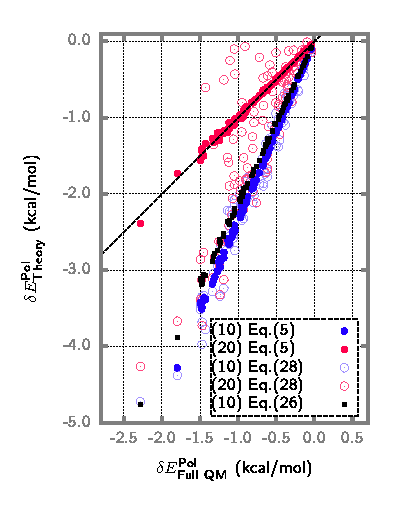
\includegraphics[width=\textwidth]{data/dmatpol/water/figure1/fig-1.eps}
\caption{\label{f:results} {\bf Performance of the distributed density matrix susceptibility tensors in moderate
electric fields.}
Calculations of the electric field\hyp{}induced interaction energies (A-C), dipole moments (D-F) and
quadrupole moments (G-I).}
\end{figure*}
%
%\begin{table*}[]
%\centering
%\caption{My caption}
%\label{t:results}
%\resizebox{\textwidth}{!}{%
%\begin{tabular}{|l|c|c|c|c|c|c|c|}
%\hline
%\textbf{}                                                                           & \multicolumn{1}{l|}{} & \textbf{An Initio DMS} & \multicolumn{4}{c|}{\textbf{Generalized DMS}}                 & \textbf{Multipole} \\ \hline
%\textbf{}                                                                           & \textbf{Set}          & \textbf{1, 0}          & \textbf{1, 0} & \textbf{2, 0} & \textbf{1, 1} & \textbf{2, 1} & \textbf{-}         \\ \hline
%\multirow{3}{*}{\textbf{\begin{tabular}[c]{@{}l@{}}RMSE\\ (kcal/mol)\end{tabular}}} & W                     & 0.067 (99.80)          & 0.076 (99.74) & 0.053 (99.88) & 0.074 (99.76) & 0.050 (99.89) & 0.004 (100.00)     \\ \cline{2-8} 
%                                                                                    & M                     & 1.07 (96.96)           & 1.24 (95.96)  & 0.86 (98.06)  & 1.20 (96.17)  & 0.81 (98.27)  & 0.07 (99.99)       \\ \cline{2-8} 
%                                                                                    & S                     & 4.22 (88.87)           & 5.15 (83.44)  & 3.60 (91.92)  & 5.02 (84.25)  & 3.41 (92.73)  & 0.33 (99.93)       \\ \hline
%\multirow{3}{*}{\textbf{\begin{tabular}[c]{@{}l@{}}RMSD\\ (mD)\end{tabular}}}       & W                     & 3.36 (98.70)           & 1.03 (99.88)  & 0.98 (99.89)  & 0.52 (99.97)  & 0.47 (99.98)  & 3.36 (98.70)       \\ \cline{2-8} 
%                                                                                    & M                     & 14.72 (98.50)          & 7.72 (99.59)  & 6.86 (99.67)  & 6.15 (99.74)  & 5.38 (99.80)  & 14.72 (98.50)      \\ \cline{2-8} 
%                                                                                    & S                     & 44.80 (96.92)          & 33.06 (98.32) & 29.49 (98.67) & 28.74 (98.73) & 26.25 (98.94) & 44.80 (96.92)      \\ \hline
%\multirow{3}{*}{\textbf{\begin{tabular}[c]{@{}l@{}}RMSQ\\ (DA10-3)\end{tabular}}}   & W                     & 6.22 (58.72)           & 1.59 (97.32)  & 1.49 (97.62)  & 0.58 (99.64)  & 0.48 (99.75)  & 5.45 (68.30)       \\ \cline{2-8} 
%                                                                                    & M                     & 28.22 (53.90)          & 10.45 (93.68) & 8.83 (95.49)  & 8.25 (96.06)  & 6.57 (97.50)  & 23.94 (66.83)      \\ \cline{2-8} 
%                                                                                    & S                     & 78.07 (40.53)          & 43.33 (81.68) & 35.73 (87.55) & 38.80 (85.31) & 31.59 (90.26) & 64.33 (59.62)      \\ \hline
%\end{tabular}%
%}
%\end{table*}
%We first test the accuracy of the density matrix susceptibility tensors that were derived
%in Eq.~\eqref{e:susceptibility-B} from first principles. 
%For this purpose we have considered a water molecule 
%under weak uniform electric fields (Figure~XXX). 
%3D difference one\hyp{}electron density isosurface plots for sample electric fields
%with respect to the unperturbed density (${\bf F} = {\bf 0}$)
%are shown in Figure~XXX. The statistical evaluation of errors for a set of
%100 random electric fields is shown in Figure~XXX. The shape of the basins 
%of decreased/increased density are comparable with the exact result
%obtained from HF/6-311++G** calculations. 
%It can be seen that the theory
%describes the polarization of the electron density distribution qualitatively well:
%However, the accuracy in the density matrix elements is on overall very low which 
%manifests with drammatic errors in the electronic total energy of the system.
%It is due to the approximations used to derive Eq.~\eqref{e:susceptibility-B},
%which neglects quadrupole and higher\hyp{}order induced multipole moments.

%\subsection{General Model of Densty Matrix Polarization}

%However, Eq.~\eqref{e:final-model} is an approximation because (i) it is based on the approximate
%relation in Eq.~\eqref{e:dmu-l-vector-mo-transform} and (ii) only total dipole moment (but not quadrupole
%and higher moments) is exactly
%reproduced by the current model. Due to the above reasons, the existence of ${\bf X}$ that




%The critical assessment of the proposed model is discussed in two stages: (i) first
%the capability of the model in capturing the polarization 
%It is instructive to analyze first the capability of the model in capturing the polarization
%process by studying the 3D electronic density distortions due to the electric field perturbation.
%For this purpose we consider a , i.e., without
%optimization of the particular density matrix elements with respect to benchmark. 

%For this purpose we studied few molecules
%in a uniform external electric field. Although the density matrix elements in a chosen AO basis
%can be inconsistent with other quantities (such as Fock matrix and so on) the polarization 


\section{\label{s:5}Summary and a few concluding remarks}

In this Work, the \emph{ab initio} model of the one\hyp{}particle density matrix susceptibility tensors
at the HF level was derived for a closed shell molecule in a spatially non\hyp{}uniform
electric field distribution. It was found that the change in the density matrix element
is approximately proportional to the electric field evaluated at the distributed site associated with the 
center of charge of the 
localized molecular orbital. Subsequently, the \emph{ab initio} model served as a basis
for the formulation of the generalized model that is, in principle, not limited to the HF theory,
and takes into account higher\hyp{}order curvatures of the electric field distribution as well.
The generalized model consisted of a set of adjustable parameters defining the density matrix susceptibility tensors
that are able to interact with the electric field, square of electric field and electric field gradients.
The particular density matrix susceptibilities were determined through the least\hyp{}squares 
linear regression with respect to the training enseble of electrostatically perturbed states.

The above theoretically developed models were then used to calculate the electric field\hyp{}induced
interaction energies, dipole moments and quadrupole moments of water molecule that
interacts with various point charge environments generating electric fields of weak, moderate
and strong magnitudes. It was found that, while the \emph{ab initio} model yelds qualitatively correct
interaction energies and dipole moments, the generalized model can reach quantitative level of accuracy
for prediction of interaction energies, dipole moments and even quadrupole moments. Although 
errors in interaction energies produced by using the generalized model 
were still at best one order of magnitude larger than the errors produced by using the
usual approach based on the distributed polarizabilities, this work demonstrated that it is possible to
accurately predict the change in the density matrix of electronic system, and the accuracy of the model
can be improved by extending the parameter space of the susceptibility tensors. 

It is anticipated here that the generalized models from Eq.~\eqref{e:final-model.General}
should be studied in the future with an emphasis 
on their further optimization, especially to reach RMSE below 1 kcal/mole
in strong and very strong electric fields (0.05-0.07 a.u.). 
For this purpose, more general forms of Eq.~\eqref{e:final-model.General}, as well as the choice of distributed
sites should be further investigated, preferably with post\hyp{}Hartree\hyp{}Fock methods.
Nevertheless, owing the capability of the proposed approach to correctly capture the 
environment\hyp{}induced changes in the one\hyp{}particle density matrix, 
the generalized density matrix susceptibility tensors 
could be used in accurate fragment\hyp{}based calculations of extended molecular aggregates
described at correlated levels of theory, particularly including the excited state chemistry.

\begin{acknowledgments}
This project is carried out under POLONEZ programme which has received funding from the European Union's
Horizon~2020 research and innovation programme under the Marie Skłodowska-Curie grant agreement 
No.~665778. This project is funded by National Science Centre, Poland 
(grant~no. 2016/23/P/ST4/01720) within the POLONEZ 3 fellowship.
\end{acknowledgments}

%
\appendix

\section{\label{a:orig-dep} Origin-Independence of the Induced Dipole Moment}

We need to be aware that multipole integrals depend on the origin with respect to which they are evaluated.
However, the induced dipole moments defined in Eq.~\eqref{e:dmu-4-exact.linear-approximation} 
(or equivalently in Eq.~\eqref{e:dmu-l-vector})
have to be origin independent. 
%Let us check if this is the case.

Let us start with noticing that
%
\begin{equation}
 \left[ \widetilde{\mathbb{M}} \right]_{i\alpha} ({\bf r}_Q) 
 = \left[ \widetilde{\mathbb{M}} \right]_{i\alpha} ({\bf 0}) - {\bf r}_Q \left[ {\bf C}^\dagger \right]_{i\alpha}  \;.
\end{equation}
%
Further we have
%
\begin{equation}
 \left[ \widetilde{\mathbb{K}} \right]_{i\alpha} ({\bf r}_Q) 
 = \left[ \widetilde{\mathbb{K}} \right]_{i\alpha} ({\bf 0}) - {\bf r}_Q \left[ {\bf C}^\dagger {\bf D} \right]_{i\alpha} \;.
\end{equation}
%
But ${\bf C}^\dagger {\bf D}={\bf C}^\dagger {\bf C} {\bf C}^\dagger={\bf C}^\dagger$ in orthogonal
AO basis. This implies that
%
\begin{multline}
   \left[ \widetilde{\mathbb{L}} \right]_{i\alpha} ({\bf r}_Q) 
 = \left[ \widetilde{\mathbb{M}} \right]_{i\alpha} ({\bf r}_Q) 
 - \left[ \widetilde{\mathbb{K}} \right]_{i\alpha} ({\bf r}_Q) \\
 = \left[ \widetilde{\mathbb{M}} \right]_{i\alpha} ({\bf 0})   
 - \left[ \widetilde{\mathbb{K}} \right]_{i\alpha} ({\bf 0})
 = \left[ \widetilde{\mathbb{L}} \right]_{i\alpha} ({\bf 0}) \;.
\end{multline}
%
Therefore, it is proved that the polarization\hyp{}induced distributed dipole moments 
defined in Eq.~\eqref{e:dmu-4-exact.linear-approximation} 
are origin independent.
Thus, one can compute dipole integrals with respect to any origin and resulting
susceptibilities ${\bf B}_{\alpha\beta}^{(i)}$ from Eq.~\eqref{e:susceptibility-B} will be uniquely defined.

\section{\label{a:blocks} Explicit Formulae for Gradient and Hessian Blocks}

The gradient vector ${\bf g}$ and Hessian matrix ${\bf H}$ 
are build from blocks associated with the type of parameters, i.e.,
%
\begin{equation}\label{e:Newton.gH}
 {\bf g} = 
\begin{pmatrix}
{\bf g}^{[1]} \\ 
{\bf g}^{[2]} \\ 
{\bf g}^{[3]}
\end{pmatrix} ,\quad
 {\bf H} = 
\begin{pmatrix}
{\bf H}^{[11]} & {\bf H}^{[12]} & {\bf H}^{[13]} \\ 
{\bf H}^{[21]} & {\bf H}^{[22]} & {\bf H}^{[23]} \\ 
{\bf H}^{[31]} & {\bf H}^{[32]} & {\bf H}^{[33]} 
\end{pmatrix} \;.
\end{equation}
%
The gradient element of the $r$th block and Hessian element of the $(rs)$th block read
%
\begin{subequations}
 \begin{align}
  g^{[r ]}_{kv}    &\equiv \frac{\partial   Z}{\partial S_{kv}^{[r]}} 
     =-2\sum_N \overline{\delta D}^{(N)}
               \frac{\partial   \left[ \delta D^{(N)} \right]}{\partial S_{kv}^{[r]}} \;,\\
  H^{[rs]}_{kv,lw} &\equiv \frac{\partial^2 Z}{\partial S_{kv}^{[r]} \partial S_{lw}^{[s]}}  
     = 2\sum_N 
        \frac{\partial   \left[ \delta D^{(N)} \right]}{\partial S_{kv}^{[r]}}
        \frac{\partial   \left[ \delta D^{(N)} \right]}{\partial S_{lw}^{[s]}} \;.
 \end{align}
\end{subequations}
%
Note that the second derivatives of $\delta D^{(N)}$ vanish
due to the linearity with respect to the adjustable parameters.
Thus, the explicit formulae for the gradient are
%
\begin{subequations}
 \begin{align}
  g^{[1]}_{kv} &=-2\sum_N \overline{\delta D}^{(N)} F^{(N)}_{kv} \;,\\
  g^{[2]}_{kv} &=-4\sum_N \overline{\delta D}^{(N)} F^{(N)}_{kv} \widetilde{F}^{(N)}_k \;,\\
  g^{[3]}_{kv} &=-4\sum_N \overline{\delta D}^{(N)} \widetilde{F}^{(N)}_{kv} \;.
 \end{align}
\end{subequations}
%
The Hessian subsequently follows to be
%
\begin{subequations}
 \begin{align}
  H^{[11]}_{kv,lw} &= 2\sum_N F^{(N)}_{kv} F^{(N)}_{lw} \;,\\
  H^{[22]}_{kv,lw} &= 8\sum_N F^{(N)}_{kv} F^{(N)}_{lw} \widetilde{F}^{(N)}_k \widetilde{F}^{(N)}_l \;,\\
  H^{[33]}_{kv,lw} &= 8\sum_N \widetilde{F}^{(N)}_{kv} \widetilde{F}^{(N)}_{lw} \;,\\
  H^{[12]}_{kv,lw} &= 4\sum_N F^{(N)}_{kv} F^{(N)}_{lw} \widetilde{F}^{(N)}_l \;,\\
  H^{[13]}_{kv,lw} &= 4\sum_N F^{(N)}_{kv} \widetilde{F}^{(N)}_{lw} \;,\\
  H^{[23]}_{kv,lw} &= 8\sum_N F^{(N)}_{kv} \widetilde{F}^{(N)}_k \widetilde{F}^{(N)}_{lw} \;.
 \end{align}
\end{subequations}
%
In the above equations, the auxiliary quantities $\widetilde{F}^{(N)}_k$ 
and $\widetilde{F}^{(N)}_{kv}$ are defined as
%
\begin{subequations}
 \begin{align}
  \widetilde{F}^{(N)}_k    &\equiv \sum_w F^{(N)}_{kw} \;,\\
  \widetilde{F}^{(N)}_{kv} &\equiv \sum_w F^{(N)}_{kw,kv} \;.
 \end{align}
\end{subequations}
%
Note that due to the symmetry of the Hessian matrix, the blocks $21$, $31$ and $32$
are transposes of the blocks $12$, $13$ and $23$, respectively. The composite index
can be defined as $kv \equiv 3k+v$, for example.
\bibliography{references}

\end{document}
